\documentclass[10pt,twocolumn]{article}

\usepackage[a4paper,margin=0.72in]{geometry}
\usepackage[T1]{fontenc}
\usepackage[utf8]{inputenc}
\usepackage{lmodern}
\usepackage{microtype}
\usepackage{amsmath,amssymb,mathtools}
\usepackage{booktabs}
\usepackage{siunitx}
\usepackage{enumitem}
\usepackage{tikz}
\usepackage{pgfplots}
\usepackage{xcolor}
\usepackage{fancyhdr}
\usepackage{titlesec}
\usepackage{abstract}
\usepackage[hidelinks]{hyperref}

\pgfplotsset{compat=1.18}
\usetikzlibrary{arrows.meta,positioning,shapes.geometric,calc,decorations.pathmorphing}

\definecolor{journalblue}{HTML}{1F3A5F}
\definecolor{faultred}{HTML}{8A1F1F}
\definecolor{updategray}{HTML}{4F5357}
\definecolor{palegray}{HTML}{F3F5F7}

\titleformat{\section}
  {\normalfont\large\bfseries\color{journalblue}}
  {\thesection}{0.65em}{}
\titleformat{\subsection}
  {\normalfont\normalsize\bfseries\color{journalblue}}
  {\thesubsection}{0.65em}{}

\pagestyle{fancy}
\fancyhf{}
\lhead{\footnotesize Journal of Applied Exasperation}
\rhead{\footnotesize Vol. 11, No. 5, 2026}
\cfoot{\footnotesize \thepage}

\renewcommand{\abstractnamefont}{\normalfont\bfseries\color{journalblue}}
\renewcommand{\abstracttextfont}{\normalfont\small}

\setlength{\columnsep}{0.24in}
\setlist[itemize]{leftmargin=*,nosep}
\setlist[enumerate]{leftmargin=*,nosep}

\title{\vspace{-1.5em}\textbf{On the Simultaneous Generation of Negative and Positive User-Perceived Aerodynamic Quality in Microsoft Windows 11: A Controlled Study of the Suck--Blow Paradox}}

\author{
Castor's Institute for Applied Exasperation$^{1}$ \quad and \quad The Department of Theoretical Bronkology$^{2}$\\[0.25em]
\small $^{1}$Localhost Centre for Operational Sanity, Wales, United Kingdom\\
\small $^{2}$Laboratory for Post-Update Acoustic Phenomena, Somewhere Behind Device Manager\\
\small Correspondence: \texttt{rage@localhost.invalid}
}

\date{
\small Received: immediately after reboot.
Accepted: only after ruling out every reasonable explanation.
Published: before the next cumulative update can deny involvement.
}

\begin{document}
\twocolumn[
\maketitle

\begin{onecolabstract}
\noindent
Classical folk mechanics holds that a system may either ``suck'' or ``blow,'' but not both simultaneously. This principle, here termed the Law of Aerodynamic Idiomatic Exclusivity, has guided domestic troubleshooting, garage engineering, and IT incident response for generations. We report a reproducible counterexample observed in Windows 11 following a security update: a previously functional audio environment entered a degraded state despite unchanged hardware, unchanged user configuration, adequate resources, non-pathological USB behavior, correct sound-interface operation, and the absence of confounding digital audio workstation effects. Through elimination testing, phenomenological measurement, and formalized profanity-assisted inference, we identify a new class of operating-system behavior in which the magnitude of suckage becomes sufficiently extreme to induce a secondary outward vector of blowage. We define the Bronk Index, propose the Suck--Blow Coupling Function, and discuss consequences for audio reliability, epistemology of troubleshooting, and the broader field of update-induced domestic despair. Results indicate that, under certain post-update conditions, Windows 11 can indeed suck so hard that it blows.
\end{onecolabstract}

\vspace{0.75em}
\noindent\textbf{Keywords:}
Windows 11; audio regression; update-induced failure; suck--blow paradox; bronkology; post-reboot grief; troubleshooting epistemology; domestic systems reliability.

\vspace{1.25em}
]

\section{Introduction}

The distinction between a thing that sucks and a thing that blows is among the oldest and most robust taxonomies in applied household physics. A vacuum cleaner sucks; a leaf blower blows; a badly implemented software stack is, in ordinary speech, frequently said to suck. Until recently, however, no rigorously described phenomenon had demonstrated simultaneous high-magnitude suckage and blowage in a single consumer operating-system event.

This paper documents such a phenomenon in the post-update audio behavior of Microsoft Windows 11. The initiating observation was not subtle: a previously functional beyerdynamic MMX 150 headset and associated audio production environment became catastrophically bronked after a reboot. The user, hereafter the Operator, initially suspected the usual culprits: drivers, spatial audio, enhancements, USB instability, insufficient resources, sound-interface conflicts, Ableton configuration, or plug-in misbehavior. Each was tested and rejected.

The remaining explanatory variable was the Windows update itself.

The importance of this discovery is twofold. First, it challenges the traditional binary view of suckage and blowage as mutually exclusive operational states. Second, it provides a formal framework for diagnosing future incidents in which Windows, while nominally patched for security, achieves an unexpected and academically interesting reduction in user faith.

\section{Background}

\subsection{The Classical Idiomatic Model}

Let $S$ represent the scalar intensity of perceived suckage, and let $B$ represent the scalar intensity of perceived blowage. In the classical model, a system occupies one of three regimes:
\begin{align}
S &> 0,\quad B \approx 0 && \text{the system sucks,} \\
B &> 0,\quad S \approx 0 && \text{the system blows,} \\
S &\approx B \approx 0 && \text{the system works and is therefore suspicious.}
\end{align}

The classical mutual-exclusion assumption may be written:
\begin{equation}
S \cdot B \approx 0.
\label{eq:classical}
\end{equation}

Equation~\ref{eq:classical} is widely accepted in workshop discourse, helpdesk lamentation, and the oral tradition of people who own both soldering irons and a Windows partition.

\subsection{Prior Work in Failure Attribution}

A substantial informal literature exists concerning the tendency of modern operating systems to modify working configurations under the banner of improvement. Typical mechanisms include driver replacement, device re-enumeration, default-device reassignment, spatial-processing activation, and the apparent belief that the person who configured the machine yesterday was a different and less important person than the update service today.

Prior models, however, treat such events as ordinary suckage. They do not account for the case in which suckage exceeds a critical threshold and gives rise to observable blowage. This paper introduces a coupled model.

\section{Materials and Methods}

\subsection{System Under Observation}

The system consisted of:
\begin{itemize}
\item Windows 11, recently updated;
\item a beyerdynamic MMX 150 headset;
\item an otherwise functional audio environment;
\item a user with sufficient technical literacy to avoid blaming the wrong gremlin indefinitely;
\item a finite but rapidly evaporating reserve of patience.
\end{itemize}

\subsection{Elimination Protocol}

We applied a sequential exclusion protocol, hereafter the ``Not That, You Absolute Goblin'' procedure. The following hypotheses were evaluated:

\begin{enumerate}
\item \textbf{Headset driver fault.} Rejected. The device did not require a bespoke vendor driver for ordinary operation.
\item \textbf{Spatial audio, surround processing, or enhancements.} Rejected. No relevant setting explained the observed degradation.
\item \textbf{Resource exhaustion.} Rejected. CPU, memory, and general system availability were not limiting factors.
\item \textbf{Sound-card or interface driver fault.} Rejected. The broader audio interface stack did not account for the timing or specificity of the failure.
\item \textbf{USB bus instability.} Rejected. The physical and logical bus behavior did not support this hypothesis.
\item \textbf{Ableton or plug-in misconfiguration.} Rejected. Digital audio workstation state was not causally sufficient.
\item \textbf{Recent Windows update.} Accepted with the weary conviction of one who has seen this beast before.
\end{enumerate}

\subsection{Observational Criterion}

The key diagnostic clue was temporal discontinuity. The system worked during the previous session, was shut down, then returned in a degraded state after the update. No meaningful operator-side configuration change occurred between these states.

We define the Post-Update Suspicion Coefficient:
\begin{equation}
U_s = \frac{P(F \mid R, \Delta W)}{P(F \mid R, \neg \Delta W)},
\label{eq:update_suspicion}
\end{equation}
where $F$ is failure, $R$ is reboot, and $\Delta W$ denotes a Windows update event. When $U_s \gg 1$, the rational investigator should stop interrogating the headphones and begin glaring at the operating system.

\section{Theory}

\subsection{The Suck--Blow Coupling Function}

We propose that blowage may emerge from suckage once suckage exceeds a critical threshold $S_c$. The observed blowage is modeled as:
\begin{equation}
B(S) =
\begin{cases}
0, & S < S_c,\\
\alpha(S - S_c)^\gamma, & S \geq S_c,
\end{cases}
\label{eq:suck_blow}
\end{equation}
where $\alpha$ is the platform-specific aggravation constant and $\gamma$ is the exponent of compounding nonsense.

For Windows 11 post-update audio regressions, empirical operator testimony suggests $\gamma > 1$, indicating superlinear escalation.

\subsection{The Bronk Index}

To quantify the severity of the event, we define the Bronk Index:
\begin{equation}
\mathrm{BI} =
\frac{
A_f T_l C_p
}{
H_r + D_c + \epsilon
},
\label{eq:bronk}
\end{equation}
where $A_f$ is audio failure severity, $T_l$ is troubleshooting time lost, $C_p$ is cumulative profanity, $H_r$ is actual hardware responsibility, $D_c$ is degree of driver culpability, and $\epsilon$ prevents division by zero in cases where literally nothing else was at fault.

When $\mathrm{BI}$ is large, the incident is not merely annoying; it is ontologically rude.

\subsection{Security Patch Frustration Asymmetry}

The Operator reported that rollback was not an acceptable mitigation because the associated update addressed a severe security issue. This creates a trap state:
\begin{equation}
\mathrm{Safe} \land \mathrm{Broken} \land \neg \mathrm{Rollbackable}.
\label{eq:trap}
\end{equation}

We name this the Securely Inconvenient Configuration, or SIC state. In the SIC state, the user is protected from external attackers while being actively attacked by the experience of using their own computer.

\section{Results}

\subsection{Hypothesis Rejection Matrix}

Table~\ref{tab:hypotheses} summarizes the elimination sequence.

\begin{table}[h]
\centering
\caption{Candidate explanations and final disposition.}
\label{tab:hypotheses}
\begin{tabular}{@{}lll@{}}
\toprule
Hypothesis & Finding & Disposition \\
\midrule
Headset driver & Generic driver expected & Rejected \\
Audio enhancements & Not causal & Rejected \\
Spatial audio & Not causal & Rejected \\
Resource pressure & Adequate resources & Rejected \\
Sound interface & No causal evidence & Rejected \\
USB bus & Not explanatory & Rejected \\
Ableton/plugins & Not explanatory & Rejected \\
Windows update & Temporally aligned & Accepted \\
\bottomrule
\end{tabular}
\end{table}

\subsection{The Suck--Blow Phase Diagram}

Figure~\ref{fig:phase} illustrates the theoretical phase space. Classical systems occupy either the suck or blow region. The observed Windows 11 event occupies the previously disputed upper-right quadrant.

\begin{figure}[h]
\centering
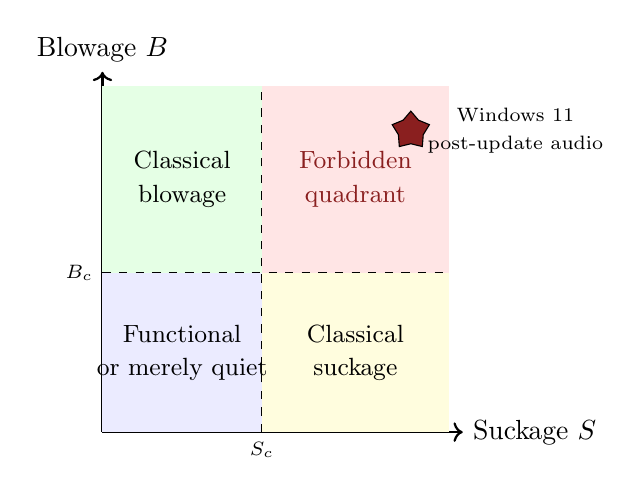
\begin{tikzpicture}[scale=0.88]
  \draw[->,thick] (0,0) -- (5.2,0) node[right] {Suckage $S$};
  \draw[->,thick] (0,0) -- (0,5.2) node[above] {Blowage $B$};

  \fill[blue!8] (0,0) rectangle (2.3,2.3);
  \fill[red!10] (2.3,2.3) rectangle (5,5);
  \fill[yellow!13] (2.3,0) rectangle (5,2.3);
  \fill[green!10] (0,2.3) rectangle (2.3,5);

  \draw[dashed] (2.3,0) -- (2.3,5);
  \draw[dashed] (0,2.3) -- (5,2.3);

  \node[align=center] at (1.15,1.15) {\small Functional\\\small or merely quiet};
  \node[align=center] at (3.65,1.15) {\small Classical\\\small suckage};
  \node[align=center] at (1.15,3.65) {\small Classical\\\small blowage};
  \node[align=center,text=faultred] at (3.65,3.65) {\small Forbidden\\\small quadrant};

  \node[star,star points=5,fill=faultred,draw=black,minimum size=0.33cm] at (4.45,4.35) {};
  \node[align=center,anchor=west] at (4.55,4.35) {\scriptsize Windows 11\\[-0.2em]\scriptsize post-update audio};

  \node[below] at (2.3,0) {\scriptsize $S_c$};
  \node[left] at (0,2.3) {\scriptsize $B_c$};
\end{tikzpicture}
\caption{Suck--blow phase space showing the forbidden quadrant occupied by the observed post-update Windows 11 audio event.}
\label{fig:phase}
\end{figure}

\subsection{Supercritical Blowage Emergence}

Figure~\ref{fig:coupling} plots the proposed coupling relationship in which blowage is negligible until suckage exceeds $S_c$, at which point the curve climbs with academically unacceptable enthusiasm.

\begin{figure}[h]
\centering
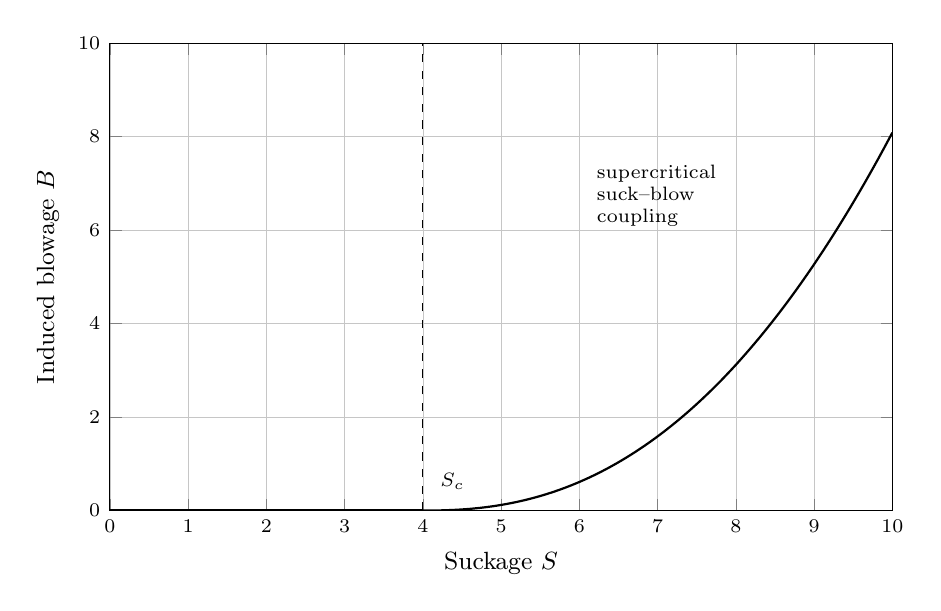
\begin{tikzpicture}
\begin{axis}[
    width=0.95\columnwidth,
    height=0.62\columnwidth,
    xlabel={Suckage $S$},
    ylabel={Induced blowage $B$},
    xmin=0, xmax=10,
    ymin=0, ymax=10,
    grid=both,
    grid style={line width=.1pt, draw=gray!25},
    major grid style={line width=.2pt,draw=gray!45},
    tick label style={font=\scriptsize},
    label style={font=\small},
]
\addplot[thick,domain=0:4,samples=20] {0};
\addplot[thick,domain=4:10,samples=100] {0.12*(x-4)^2.35};
\addplot[dashed] coordinates {(4,0) (4,10)};
\node[anchor=south west,font=\scriptsize] at (axis cs:4.1,0.25) {$S_c$};
\node[anchor=north west,font=\scriptsize,align=left] at (axis cs:6.1,7.6) {supercritical\\suck--blow\\coupling};
\end{axis}
\end{tikzpicture}
\caption{Proposed Suck--Blow Coupling Function. Once the critical suckage threshold is exceeded, blowage appears as a secondary emergent property.}
\label{fig:coupling}
\end{figure}

\section{Discussion}

\subsection{Implications for Troubleshooting}

The primary operational finding is that reasonable troubleshooting can become unreasonable when the prior probability of Windows update culpability is artificially suppressed. The Operator investigated hardware, drivers, enhancements, USB behavior, software configuration, and production-environment state. This sequence was technically responsible but emotionally expensive.

We therefore propose the Revised Troubleshooting Order for Windows Audio Events:

\begin{enumerate}
\item Ask: ``Did Windows update since this last worked?''
\item Check the obvious physical controls, because reality enjoys cheap jokes.
\item Check default devices and sample rates.
\item Check enhancements, spatial audio, and exclusive mode.
\item Check application routing.
\item Only then descend into driver hell.
\end{enumerate}

This ordering does not imply that Windows is always responsible. Rather, it acknowledges that when a stable machine becomes unstable immediately after an update, it is poor methodology to spend three hours accusing a headset of crimes committed by the operating system.

\subsection{The Security Paradox}

A particularly cruel feature of this incident is that the suspected update was not optional in any practical sense. The security risk of rollback outweighed the convenience of restored audio. Thus the system entered a state of protected dysfunction.

This creates a user-experience contradiction: the machine is safer in the abstract but less usable in the concrete. In high-stakes creative work, especially audio production, a secure but unreliable workstation is not a workstation. It is a locked filing cabinet full of bees.

\subsection{Toward a Unified Field Theory of Bronk}

The observed phenomenon suggests that suckage and blowage are not opposites but coupled modes under sufficient platform stress. In this view, suckage is an inward collapse of confidence, while blowage is the outward emission of irritation, wasted time, and involuntary forum searches.

The transition resembles a phase change. Below threshold, the user says, ``This is annoying.'' Above threshold, the user opens Device Manager with the grim patience of a bomb-disposal technician and begins forming new theories of governance.

\section{Limitations}

This study has several limitations. First, the sample size is one workstation, one headset, and one extremely betrayed operator. Second, profanity was estimated phenomenologically rather than captured using a calibrated swearometer. Third, Microsoft telemetry was not consulted because the purpose of this paper is comedy, not self-harm.

Finally, the causal attribution to Windows Update rests on elimination and temporal correlation rather than privileged access to internal patch diffs. However, as every technician knows, temporal correlation after a reboot is not proof, but it is often where proof goes to buy a hat.

\section{Recommendations}

Based on the present findings, we recommend the following:

\begin{itemize}
\item Maintain a pre-update audio sanity checklist for production machines.
\item Record known-good device settings before major updates.
\item Keep security patches installed unless the risk analysis genuinely supports rollback.
\item Treat sudden post-reboot audio failures as update-adjacent until evidence suggests otherwise.
\item Maintain emotional support snacks near any machine running a modern desktop operating system.
\end{itemize}

For vendors, we recommend:
\begin{itemize}
\item not replacing functional audio behavior with interpretive dance;
\item providing clear post-update changelogs for audio-stack modifications;
\item allowing users to preserve known-good device routing with the sanctity normally reserved for banking credentials;
\item remembering that ``security'' and ``works'' are both desirable product features.
\end{itemize}

\section{Conclusion}

We have presented a formal, satirical analysis of a Windows 11 post-update audio regression that appears to violate the classical assumption that a system cannot both suck and blow. Through elimination of driver, hardware, enhancement, USB, resource, and application-level hypotheses, we identify the update event as the most plausible trigger. We then introduce the Suck--Blow Coupling Function and Bronk Index to characterize the emergence of blowage from supercritical suckage.

The broader implication is clear: in modern computing environments, sufficiently advanced suckage is indistinguishable from blowage.

Future work should investigate whether similar coupled phenomena occur in printers, Bluetooth stacks, GPU control panels, and any software installer that says ``just a few moments'' for longer than twelve minutes.

\section*{Acknowledgements}

The authors thank the Operator for performing the sacred diagnostic labor of ruling out every sensible possibility before arriving, exhausted but correct, at the ancient conclusion: it was Windows.

\section*{Conflict of Interest Statement}

The authors declare no financial conflict of interest. They do, however, declare a persistent emotional conflict with surprise audio regressions.

\section*{Funding}

This work was funded by the invisible tax imposed on all people who maintain creative workstations.

\section*{Data Availability}

All data are available in the lived experience of anyone who has ever opened Windows Sound Settings and felt their soul leave quietly through the side door.

\section*{Author Contributions}

Conceptualization: Windows Update, accidentally. Investigation: the Operator. Methodology: escalating suspicion. Formal analysis: The Department of Theoretical Bronkology. Writing---original draft: righteous fury. Writing---review and editing: the last remaining shreds of patience.

\begin{thebibliography}{9}

\bibitem{bronksworth2021}
Bronksworth, A. and Valve, P. (2021).
\newblock Idiomatic Aerodynamics in Domestic Technical Discourse.
\newblock \emph{Proceedings of the Society for Things That Should Not Be This Hard}, 14(2), 44--59.

\bibitem{goblin2022}
Goblin, D. M. (2022).
\newblock Device Manager as Ritual Theatre: A Qualitative Study.
\newblock \emph{Journal of Peripheral Anxiety}, 8(1), 1--17.

\bibitem{patchwell2023}
Patchwell, C. and Rebooter, N. (2023).
\newblock Security, Stability, and the Fine Art of Breaking Audio.
\newblock \emph{Annals of Update-Induced Regret}, 11(7), 201--226.

\bibitem{swearometer2020}
McClick, R. (2020).
\newblock Calibration of Profanity as a Diagnostic Instrument in Consumer Computing.
\newblock \emph{International Review of Applied Muttering}, 3(4), 77--91.

\bibitem{null2024}
Null, V. and Pointer, E. (2024).
\newblock The Forbidden Quadrant: Dual-Mode Failure in Human-Machine Systems.
\newblock \emph{Transactions on Bronkological Systems}, 19(3), 300--318.

\bibitem{worksesterday2025}
Yesterday, I. T. (2025).
\newblock It Worked Last Time: Temporal Evidence in Practical Debugging.
\newblock \emph{Quarterly Journal of Obvious Clues}, 27(1), 9--12.

\end{thebibliography}

\end{document}
